
%(BEGIN_QUESTION)
% Copyright 2012, Tony R. Kuphaldt, released under the Creative Commons Attribution License (v 1.0)
% This means you may do almost anything with this work of mine, so long as you give me proper credit

Skjemaet nedenfor viser et overstrømsvernrele av typen Westinghouse CO-11, komplett med tidsforsinket overstrøm (``CO''), momentan overstrøm (``IIT'') og holdestrøms-/seal-in-element (``ICS''). Releet som er vist er tatt ut av drift og står på en arbeidsbenk klar for testing av en tekniker:

$$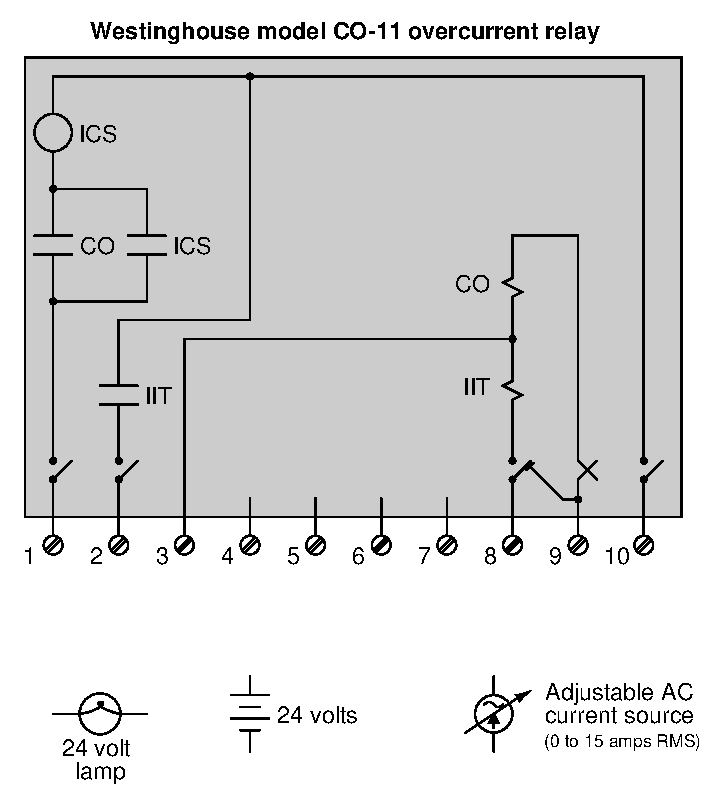
\includegraphics[width=15.5cm]{i01173x01.eps}$$

Tegn inn alle nødvendige forbindelsesledninger for å teste {\it kun} funksjonen momentan overstrøm (50). En justerbar AC-strømkilde gir innmating til releet, mens en lyspære brukes for å indikere når releets utløserkontakt(er) har sluttet.

\underbar{file i01173}
%(END_QUESTION)





%(BEGIN_ANSWER)

{\it Vurderingen er alt-eller-ingenting. Enten er kretsen koblet riktig, eller så er den ikke.}  

$$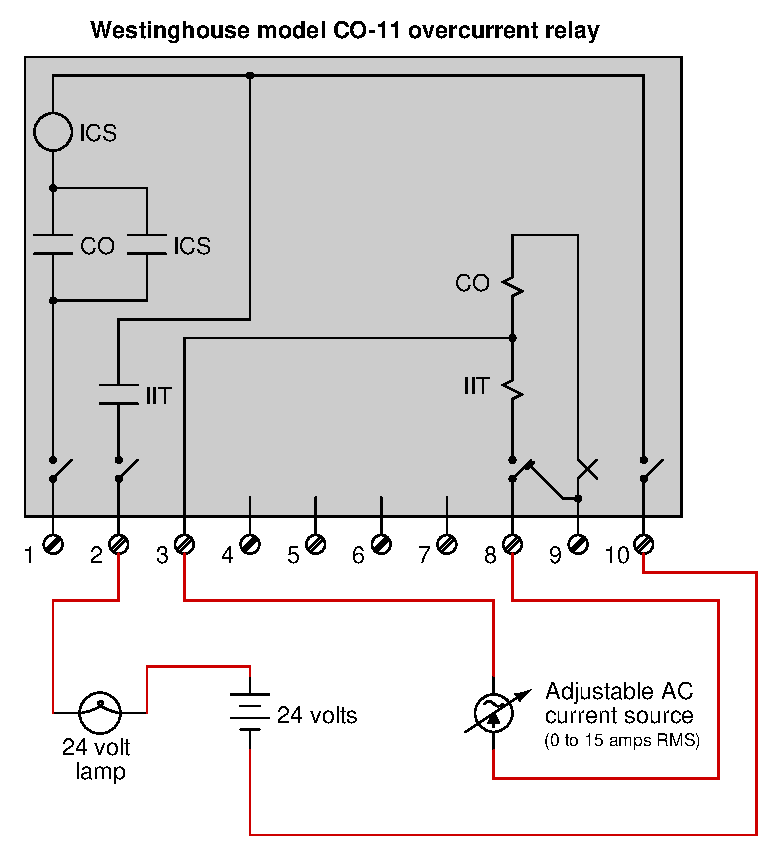
\includegraphics[width=15.5cm]{i01173x02.eps}$$

Merk: det er også tillatt å koble den justerbare AC-strømkilden til terminal 8 og 9, i stedet for 3 og 8. Dette vil energisere både CO- og IIT-spolene, men IIT-funksjonen blir fortsatt testet tilfredsstillende. Polaritet er irrelevant både for AC-teststrømkilden og for 24 VDC-utløserindikator-kretsen med lyspære.
 
%(END_ANSWER)





%(BEGIN_NOTES)

{\bf Denne oppgaven er kun ment for prøver/eksamen, ikke arbeidsark!}

%(END_NOTES)

